% Template for ICIP-2019 paper; to be used with:
%          spconf.sty  - ICASSP/ICIP LaTeX style file, and
%          IEEEbib.bst - IEEE bibliography style file.
% --------------------------------------------------------------------------
\documentclass{article}
\usepackage{spconf,amsmath,graphicx}
\usepackage{amssymb}
\usepackage[colorlinks, citecolor=blue]{hyperref}
\usepackage{multirow}
\usepackage{caption, subcaption}
\usepackage{colortbl, booktabs, array}

\setlength{\aboverulesep}{0pt}
\setlength{\belowrulesep}{0pt}

% Example definitions.
% --------------------
\def\x{{\mathbf x}}
\def\L{{\cal L}}

% Title.
% ------
\title{Robo-Advisor using BERT sentiments from Tweets for hybrid Portfolio Optimisation with Genetic Algorithm}
%
% Single address.
% ---------------
\name{Edmund Leow Kwong Wei, Matthew Chua Chin Heng}
\address{Institute of Systems Science, National University of Singapore, Singapore 119615}

\begin{document}
%\ninept
%
\maketitle
%
\begin{abstract}

Robo-advisors are increasingly popular, with machine learning algorithms taking centre stage for researchers. However, classical financial theories and techniques, such as Constant Rebalancing (CRB) and Modern Portfolio Theory (MPT), can still be relevant by combining them with social media sentiments. In this study, we propose the so-called Sentimental All-Weather (SAW) and Sentimental MPT (SMPT) models which capture the up-to-date market conditions through Twitter sentiments. Trained on tweets and US stock data from August 2018 to end December 2019, our experiments reveal that the proposed models can achieve superior performance in terms of common measures of portfolio performance (such as Sharpe ratio, cumulative returns, value-at-risk), compared to the following benchmarks: buy-and-hold SPY index, MPT model, and CRB model for an All-Weather Portfolio, for out-of-sample period from January 2020 to April 2020.

\end{abstract}
%
\begin{keywords}
portfolio optimisation, genetic algorithm, Social media sentiment analysis
\end{keywords}
%
\section{Introduction}

Innovations in financial technology (FinTech) are driving the banking sector, with more changes expected in the next couple of years than in the past two centuries \cite{morechanges10}. One of the most important changes is the introduction of advanced technology, such as machine learning algorithms, to facilitate security trading and advisory services to investors, collectively termed robo-advisors \cite{roboadvisors_wealth}.

The opportunity for robo-advisors is tremendous as it enables small investors to gain entry to low-fee automated wealth management, with low-minimum investment requirements \cite{rise_robo}. Another key advantage of robo-advisors is that they are less vulnerable to potential conflicts of interest, because they provide significantly lower and more transparent cost structures, compared to human financial advisors who are often prone to misguided incentive-based compensation schemes \cite{BRENNER2020100275}.

In recent years, several studies \cite{GOMES200143} have shown that artificial intelligence can achieve better portfolio management performance than using existing strategies based on classical financial theories and traditional models, such as Modern Portfolio Theory (MPT) \cite{markowitz_1991}, and Hierarchical Risk Parity (HRP) \cite{hrp}. However, the decisions of machine learning methods in a robo-advisor are difficult or impossible to explain, which can hamper users’ trust in the system, and can lead to the rejection of the system \cite{rai2020explainable}. Most existing robo-advisors in the market also still utilise MPT, and is the method that fund managers are most familiar with \cite{lam2016robo}.

At the same time, with the proliferation of social media, sentiment analysis is a growing area of interest, and this presents an opportunity to utilise Twitter sentiments as a trading signal to augment existing portfolio algorithms \cite{peterson2016trading}.

Therefore, in this paper, we propose a hybrid approach of using traditional portfolio techniques together with Twitter sentiments to improve portfolio performance, and introduce two models - Sentimental All-Weather (SAW) and Sentimental Modern Portfolio Theory (SMPT). The use of traditional portfolio techniques as a backbone will make it easier for clients and managers alike to understand, while the addition of Twitter sentiments will make it sensitive towards potential market dips and spikes.

\section{Related work and theories}
\subsection{Stock selection and prediction}
\label{stock_selection}

In creating a portfolio, it is common to adopt diversification to reduce total variance while maintaining expected return on investment, by allocating investments across different financial instruments. It is ineffective to merely invest in a large number of different assets, but to instead focus on minimising correlation between all the assets \cite{diversification}. Common traditional methods of accomplishing the above was by allocating across either different industries/sectors (health care, real estate, utilities, etc) or different asset types (equity, bonds, commodity, etc).

For each of these classes, stocks may be selected traditionally based on key technical and fundamental features \cite{schwabbrokerage}. For long-term investments, fundamental analysis, which examines a company’s management structure, competitors, industry position, growth rate, growth potential, income, and revenues to try to determine if it is a good value, is well-suited. For short-term investments, technical analysis, which focuses on patterns within stock charts to forecast future pricing and volume trends, is often used.

In recent years, machine learning techniques have also been used for stock selection. Fu et al. \cite{fu2018machine} used Genetic Algorithm (GA) to select 114 features out of 244 technical and fundamental features, and used a variety of machine learning algorithms (Logistic regression (LR), random forest (RF), deep neural network (DNN), and stacking of RF with DNN) to classify stocks as either good or bad.

It is also common to use machine-learning models to predict stock trends and returns. Kai Chen et al. \cite{Chen2015ALM} used Long Short-Term Memory (LSTM) for China stock index prediction with low-frequency data. Yang et al. \cite{yang2019deep} used Convolutional Neural Network (CNN) and LSTM models with high-frequency price-volume data to predict the expected return rate on the current day, and select stocks with the highest expected yield at the opening to maximise total returns.

Shunrong Shen et al. \cite{shen2012stock} recognised and exploited the temporal correlation among global stock markets and various financial products to predict the next-day stock trend with the aid of support vector machine (SVM), and created a practical trading model for the stock index.

The performance of price-prediction-based algorithms depends on the degree of prediction accuracy but future market prices are difficult to predict \cite{jiang2017deep}, so many have converted the problem to a Reinforcement Learning one. Hailin Li et al. \cite{hailin2007} proposed actor-critic Reinforcement learning-based system that could forecast short-term stock price movements. Furthermore, Yue Deng et al. \cite{ddrl2016} constructed a new model, Deep Direct Reinforcement Learning (DDRL), which combined direct reinforcement learning with deep recurrent neural network, for futures contract trading.

However, all of the above machine learning approaches typically seek to maximise returns, do not compare with traditional portfolio approaches such as Modern Portfolio Theory, and do not consider other factors such as differing objectives, risk appetites, maximum draw-down etc, which we deem necessary in a robo-advisor.


\subsection{Sentiments based on financial tweets for stock prediction and rebalancing}

Due to the enormous interest and and applicability in deriving automated sentiment or polarity analysis from text using natural language processing (NLP), there has been a large number of different methods in recent years. They can be split into two main methods, namely lexical-based and supervised machine learning methods.

Lexical methods typically use a predefined list of words, where each word is associated with a specific sentiment, but are very dependent on the context which they were created for \cite{sentibench}. Some, such as Valence Aware Dictionary and sEntiment Reasoner (VADER) \cite{VADER}, also combine the lexicon with processing of sentence characteristics to determine sentence polarity.

In recent years, deep learning models, particularly Google's Bidirectional Transformer (BERT) model \cite{sun2019utilizing,xu2019bert} and its variants, have gained unprecedented popularity and set new records in NLP tasks in the \href{https://gluebenchmark.com/leaderboard}{GLUE} (General Language Understanding Evaluation) Benchmark.

In general, however, no single method always achieves the best prediction performance for all different datasets \cite{sentibench}. Therefore, whichever the method chosen, the model should be fine-tuned based on the specific dataset. Araci \cite{araci2019finbert} acknowledged that financial texts have a specialised language with unique vocabulary, and have a tendency to use vague expressions instead of easily identified negative/positive words, which make models trained on general corpora ill-suited for this purpose. Therefore, he fine-tuned BERT for financial data (FinBERT), and showed that it outperforms state-of-the-art machine learning methods for financial sentiment analysis datasets \cite{araci2019finbert}.

Commercialisation of financial sentiment analysis is also increasing, with sentiment analysis vendors such as \href{http://sentdex.com/financial-analysis/}{Sentdex}, \href{https://psychsignal.com/about}{PsychSignal}, and \href{http://docs.accern.com/#unique-stories-story_id}{Accern}, offering sentiment analysis as a service.

In utilising sentiments for stock analysis and prediction, there have been numerous research and studies. Zhang and Skiena \cite{zhang2010trading} used blogs and news data to derive company-specific sentiments which are then used to rank and shortlist top and bottom companies for a long-short strategy based on the sentiments. For social media sentiments, Bollen et al. \cite{Bollen2011} used a fuzzy neural network and showed that the public collective mood (happy, calm, anxiety) derived from Twitter are correlated to the value of the Dow Jones Industrial Index. A number of articles \cite{pagolu2016, SulTwitter2017} also found that public sentiments in tweets about specific firms were significantly related to stock market movements of the companies on subsequent days. More recently, it was also shown that strongly negative tweets from just an individual account (president Donald Trump) causes subsequent short-term reduction of market value of the company mentioned \cite{DonaldTrumpTwitter}. However, in the above approaches, there was no performance comparison of prediction with any benchmarks, and the studies mostly focused on company-specific news and prediction.

\subsection{Stock rebalancing}
A portfolio's asset allocation determines the portfolio's risk and return characteristics. To maintain its original risk and return characteristics over time, the portfolio must be rebalanced either periodically at fixed intervals (e.g. monthly, semi-annually, annually) and/or at certain trigger thresholds (e.g.exceed 5\% of desired allocation percent).

One of the simplest traditional methods for stock rebalancing is the Constant Rebalanced (CRB) portfolio, where rebalancing follows a certain percentage for each asset in the portfolio. A popular CRB is the 60/40 rule, which advocates that 60 percent of the portfolio be invested in potentially higher risk and historically higher return assets, such as stocks, and the other 40 percent in lower risk assets such as government bonds \cite{brett6040}. Another popular CRB is the simplified All-Weather portfolio by Ray Dalio, which simplifies the original All-Weather risk parity approach of four equal-risk economic seasons \cite{bridgewater} into fixed-proportion allocation (30\% stocks, 40\% long-term bonds, 15\% intermediate-term bonds, 7.5\% gold, and 7.5\% commodities) \cite{robbins_2016}.

Another method for stock rebalancing is Modern Portfolio Theory (MPT) or Mean-Variance Optimisation (MVO) \cite{markowitz_1991}, where the expected return (mean) in a universe of assets is maximised given a constraint on its risk (variance), forming the Markowitz's Efficient Frontier. However, in practice, it sometimes gave unintuitive weights that did not make sense to general investors, due to estimation errors in returns and variance \cite{xu2008black}. Hence, alternative returns and risk models were proposed by others. For instance, this was addressed by Black and Litterman \cite{Black_1991}, with the Black-Litterman model, which uses a Bayesian approach to combine a prior estimate of returns with views on certain assets, so as to produce a posterior estimate of expected returns that is more intuitive \cite{Idzorek2004}. Similarly, instead of using the raw sample covariance matrix as the risk model, Ledoit and Wolf \cite{Ledoit2004, Ledoit2001} proposed transforming it (shrinking) with a structured estimator to pull the most extreme coefficients toward more central values, systematically reducing estimation error when it matters most. These alternative returns and risk models could then be used in MPT optimisation for better performance.

A relatively new technique for stock rebalancing is Hierarchical Risk Parity \cite{hrp}, introduced by Lopez de Prado, which performs hierarchical clustering on the covariance matrix of stock returns to find a diversified weighting by distributing capital to each cluster hierarchy. This gets around the issue of inverting the covariance matrix in classic MPT optimisation.

With regard to rebalancing, machine learning techniques have also been utilised. Reinforcement learning (RL) is popular as a machine learning technique for portfolio management because the stock market price dynamics are difficult to predict using supervised and unsupervised learning paradigms. However, RL has the ability to capture the temporal difference in the signals and learn the market dynamics over time. Aboussalah and Lee \cite{SDDRRL} used Stacked Deep Dynamic Recurrent Reinforcement Learning (SDDRRL) to construct real-time rebalancing optimal portfolio based on market conditions, so as to maximise Sharpe ratio, and showed that it achieves better performance than the MPT and risk parity models after 20 successive rounds for 10 selected stocks from different sectors of the S\&P 500. Similarly, Liang et al. \cite{liang2018adversarial} used continuous reinforcement learning algorithms, namely Deep Deterministic Policy Gradient (DDPG), Proximal Policy Optimisation (PPO), and Policy Gradient (PG) for portfolio management in the China stock market.

However, deep reinforcement learning is often highly sensitive with an unstable performance, and tends to shift all holdings to one asset at a time \cite{liang2018adversarial}.

\section{Proposed approach}
\label{sec:proposed approach}

Machine learning methods are often a black box, which makes it very difficult or even impossible to explain to clients how the algorithms decided on their portfolio weights when used in a robo-advisor \cite{darksecretAI_2017}, and this inscrutability can hamper users’ trust in the system, especially in a robo-advisor where the investor's money is at stake, and can lead to the rejection of the system \cite{rai2020explainable}.


Therefore, in designing the robo-advisor, we wanted a portfolio algorithm that is
\begin{itemize}
    \setlength{\itemsep}{0pt}
    \setlength{\parskip}{0pt}
    \setlength{\parsep}{0pt}
    \item comprehensive to the average investor (should not be a black box; back-tested returns and risks should be visible)
    \item transparent - client should know what they are holding in the portfolio (i.e. holdings should not keep changing)
    \item adaptive to market conditions
    \item as simple as possible while being able to out-perform the market and traditional algorithms
\end{itemize}

Almost all prior work adopt an either-or approach, where they try to advocate a new model that is supposedly better than others. Here, we will attempt a hybrid approach, using traditional portfolio optimisation approaches as a baseline and augmenting portfolio performance using sentiments derived from Twitter. The usage of traditional portfolio optimisation as a backbone is advantageous as it is mostly familiar to investors and fund managers alike, and is easier to explain. By using Twitter sentiments as an insight into overall investor sentiments, we will also be pro-active towards potential market dips and spikes, and be able to increase our cumulative returns. An overview of the proposed approach is illustrated in Fig \ref{figure_overall}. The decision points as well as key functions will be explained in the subsequent sub-sections.

\begin{figure}[tbh]
    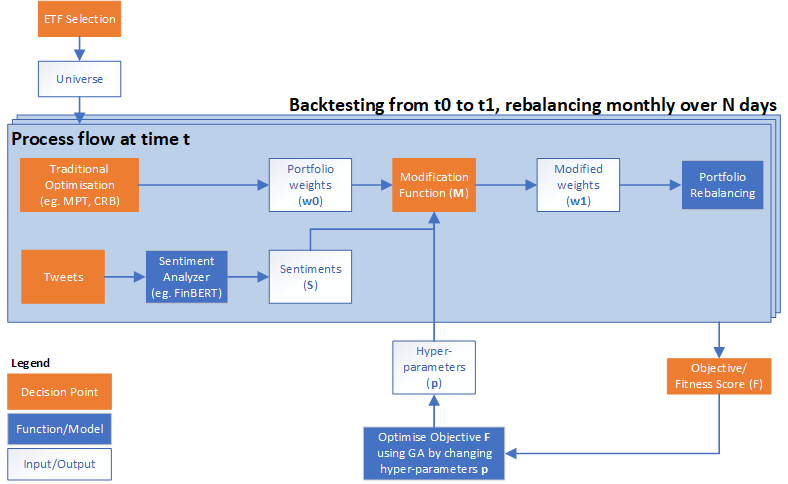
\includegraphics[width=8cm]{figure_overall_architecture.png}
    \caption{Overview of proposed hybrid approach for portfolio optimisation \label{figure_overall}}
\end{figure}

\subsection{ETF selection}

The first requirement is to choose the basket of Exchange-Traded Funds (ETFs) (universe). This is the "ETF selection" block in  Fig \ref{figure_overall}. Only US ETFs will be considered as they are ideal for automated portfolios /robo-advisors due to their broad diversification and low cost \cite{etf2002}. There are many possibilities for ETF selection as mentioned in \ref{stock_selection}, including machine learning algorithms. For simplicity, we will consider only (i) one set of ETFs for sector-based diversification and (ii) another set for asset-based diversification. These can be easily switched out with more complex stock-selection algorithms in the overall flow if required.

The sector-based basket of ETFs comprises \href{http://www.sectorspdr.com/sectorspdr/}{11 SPDR sector ETFs} (namely XLE, XLRE, XLF, XLV, XLC, XLI, XLY, XLP, XLB, XLK, XLU) which are ETFs of S\&P 500 stocks grouped by Global Industry Classification Standard (GICS) sector classification to facilitate passive investment in specific sectors of the US economy, to create a diversified portfolio across sectors (Table \ref{table_spdr}).

For asset-based diversification, we will consider the following asset classes as advocated by the All-Weather portfolio - equities, long-term bonds, intermediate-term bonds, gold, and commodities, which provide exposure to a variety of assets that perform differently across market environments. As there are many possible ETFs for each asset class, only one ETF will be taken as a representative of its asset class (Table \ref{table_all_weather}).

\begin{table}[tbh]
\caption{Symbols and sector types for SPDR ETFs}\label{table_spdr}
\centerline{
\begin{tabular}{| l | l |}
\hline
Symbol & Select sector SPDR fund\\\hline\hline
XLC & Communication Services\\\hline
XLY & Consumer Discretionary\\\hline
XLP	& Consumer Staples\\\hline
XLE	& Energy\\\hline
XLF	& Financials\\\hline
XLV	& Health Care\\\hline
XLI	& Industrials\\\hline
XLB	& Materials\\\hline
XLRE & Real Estate\\\hline
XLK	& Technology\\\hline
XLU	& Utilities\\\hline
\end{tabular}
}
\end{table}

\begin{table}[tbh]
\caption{Representative symbols and asset types for the All-Weather portfolio, as suggested by \href{https://portfolioslab.com/portfolio/ray-dalio-all-weather}{PortfoliosLab}}\label{table_all_weather}
\centerline{
\begin{tabular}{| l | l |}
\hline
Symbol & Asset Type\\\hline\hline
VTI & Equities\\\hline
TLT & Long-term bonds\\\hline
IEF	& Intermediate-term bonds\\\hline
GLD	& Gold\\\hline
DBC	& Commodities\\\hline
\end{tabular}
}
\end{table}

\subsection{Portfolio backtesting}

Backtesting simulates a trading strategy to evaluate how effective the strategy might have been if it were traded historically. The results offer statistics to gauge the effectiveness of the strategy.

Daily time-series data are obtained for the selected ETFs from \href{https://sg.finance.yahoo.com/}{Yahoo Finance}. Models are trained based on data from August 2018 to end December 2019, and backtested with out-of-sample data from January 2020 to April 2020. This allows the training and testing dataset to contain the market crash in December 2018 and the COVID-19 crash in January 2020 respectively (See Fig \ref{figure_SPY}).

Commission for trades is assumed to be USD 0.005 per share, with minimum USD 1.00 per order. This follows the pricing structure of \href{https://www1.interactivebrokers.com/en/index.php?f=1590&p=stocks}{Interactive Brokers}, the top stock broker in US.

\begin{figure}[tbh]
    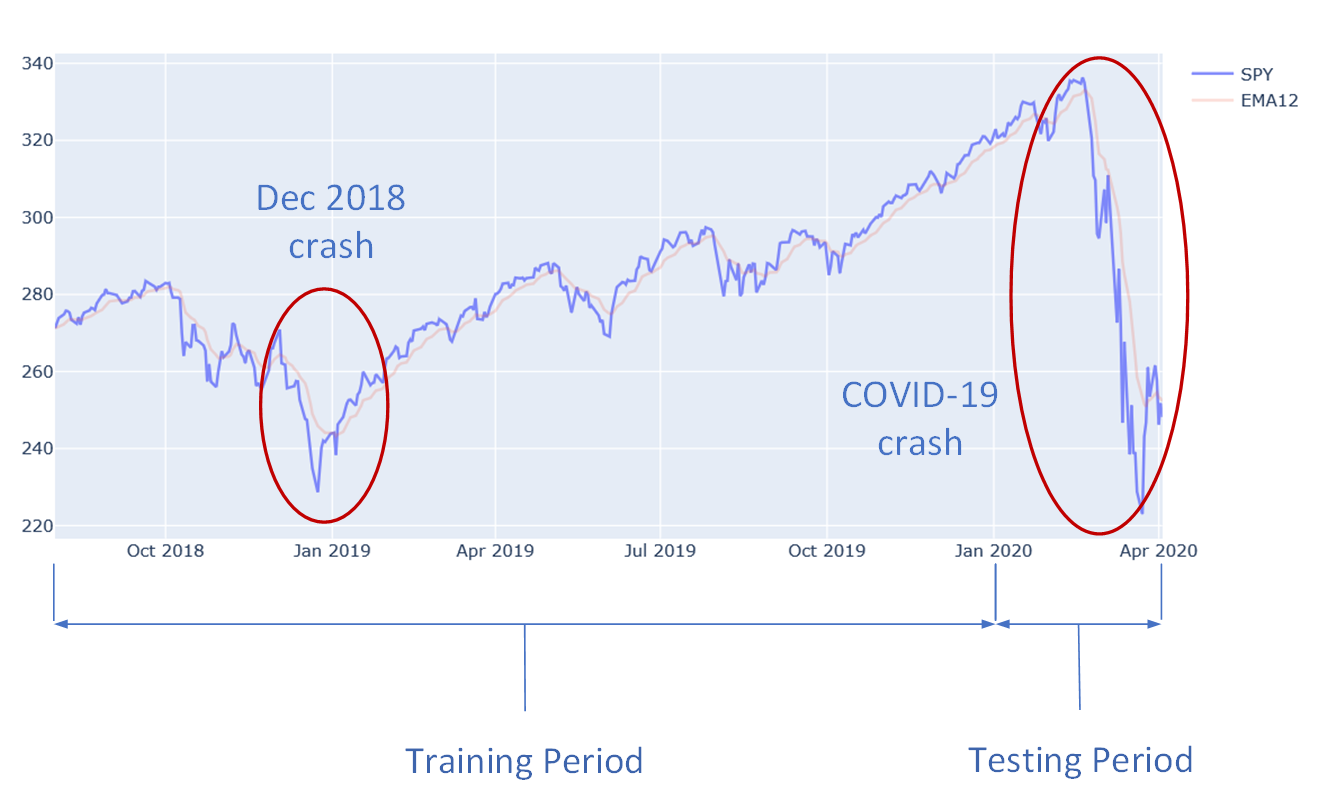
\includegraphics[width=8cm]{figure_SPY.png}
    \caption{SPDR S\&P 500 (SPY) daily closing prices for the period of August 2018 to April 2020, as representative of US stock market  \label{figure_SPY}}
\end{figure}




\subsection{Traditional optimisation and baselines}
We consider the following traditional portfolio optimisation approaches, MPT and CRB, in the "Traditional Optimisation" block in Fig \ref{figure_overall}. All rebalancing will be performed at the end of each month, and triggered only if target allocation differs from its current allocation by more than a threshold of 5\%.

For CRB, the starting weights for the SPDR ETFs follow a naive equal-weighted allocation. For the All-Weather portfolio, the starting weights are the original recommended fixed-proportion allocation (30\% stocks, 40\% long-term bonds, 15\% intermediate-term bonds, 7.5\% gold, and 7.5\% commodities) \cite{robbins_2016}.

For MPT, we use the "default textbook" mean historical returns for annualised expected returns as it is easily interpretable. Instead of using the sample covariance (S), Ledoit-Wolf shrinkage covariance matrix \cite{Ledoit2004} is used for the risk model, with an estimator given by Equation \ref{eqn_ledoit_wolf}, where F is the shrinkage target and $\delta$ is the shrinkage coefficient.

\begin{equation}
\delta F + (1-\delta)S,\ \ \ 0 \leqslant \delta \leqslant 1 \label{eqn_ledoit_wolf}
\end{equation}

All hybrid models will be baselined against a buy-and-hold strategy, as well as its corresponding traditional optimisation approach. Again, the traditional optimisation algorithms can be easily switched out with more complex variants in the overall flow if required.

\subsection{Sentiments from Twitter data}
Unlike most other work that focuses on company-specific tweets, we aim to capture the overall market sentiment, because we choose to decouple portfolio rebalancing from portfolio asset selection. This will enable us to have a fixed set of assets/holdings that will change only in terms of its percent allocation, so that our customers will be clear on what they are investing in (otherwise their holdings will likely fluctuate wildly with each rebalance). As such, we web scrape tweets from chosen specific accounts rather than filter based on mentions of companies.

For each of the chosen accounts, we web scrape the entire backtesting period, and convert each tweet into sentiments. We employ and contrast two methods, namely VADER \cite{VADER} and FinBERT \cite{araci2019finbert}.

Next, we perform post-processing, where tweets are converted to the correct timezone to correspond with the US trading market, and sentiments scores are aggregated to a per-day resolution. In order to reduce noise and outliers, we take the exponential moving average (EMA) over different spans.

Finally, we check for possible synchrony between stock data and tweet sentiments during volatile periods to shortlist suitable Twitter accounts that can represent the overall market sentiment.

\subsection{Genetic Algorithm optimisation}

We define a modification function (M) that takes in (i) EMA-weighted sentiment (S) and (ii) hyper-parameters (p), to transform traditional optimisation portfolio weight vector ($\vec{w_0}$) to modified weight vector ($\vec{w_1}$) at each rebalance interval (See Fig \ref{figure_overall}). For any given day, D, tweets and sentiments are used only up to D-1, to prevent look-ahead bias.

Applying Occam's razor, we start with the simplest possible modification functions and progressively add complexity. We calculate the Moving Average Convergence Divergence (MACD) of sentiments, $S_{cd}$, by subtracting the 26-period sentiment EMA from the 12-period EMA; and use it as a bullish signal if $S_{cd} > 0$ and as a bearish signal if $S_{cd} \leqslant 0$ (Eqn \ref{eqn_macd}).

\begin{equation} \label{eqn_macd}
S_{cd} = S_{12} - S_{26}
\end{equation}

For CRB, some of the modification functions that were attempted are shown in Table \ref{table_crb_mod}. For MPT, an intuitive modification is to modify the expected volatility. For example, if the estimation is bullish, we should be able to take more risk such that our expected return along the efficient frontier will be higher. As such, instead of directly modifying the weights from MPT, we will first get the optimal volatility from MPT, modify it with a delta and then calculate the modified weights. This can be illustrated by the Markowitz Bullet in Fig \ref{figure_smpt_markowitz}, using the All-Weather portfolio components. A couple of volatility adjustments are attempted, and the final volatility adjustment, $v_{adj}$, is calculated by Eqn \ref{eqn_smpt}.

\begin{equation} \label{eqn_smpt}
v_{adj} = \begin{cases}
  v_{mpt} * (1 +  S_{cd} * w_p), &\text{$S_{cd} > 0$}  \\
  v_{mpt} * (1 +  S_{cd} * w_n), &\text{$S_{cd} \leqslant 0$}  \\
\end{cases}
\end{equation}

\begin{table}[tbh]
\caption{Sample modification functions for CRB in order of increasing complexity. $S_n$ denotes EMA sentiment for n spans}\label{table_crb_mod}
\centerline{
\begin{tabular}{| l | l |}
\hline
Index & Equation\\\hline\hline
1 & $\vec{w_1} = \vec{w_0} * S * \vec{p}$, \\\hline
2 & $\vec{w_1} = \vec{w_0} + S * \vec{p}$, \\\hline
\multirow{2}{*}{3}   & $\vec{w_1} = \vec{w_0} + \vec{p_p}$ if $S_{12} - S_{26} > 0$\\
                     & $\vec{w_1} = \vec{w_0} + \vec{p_n}$ if $S_{12} - S_{26} \leqslant 0$\\\hline
\end{tabular}
}
\end{table}

\begin{figure}[tbh]
    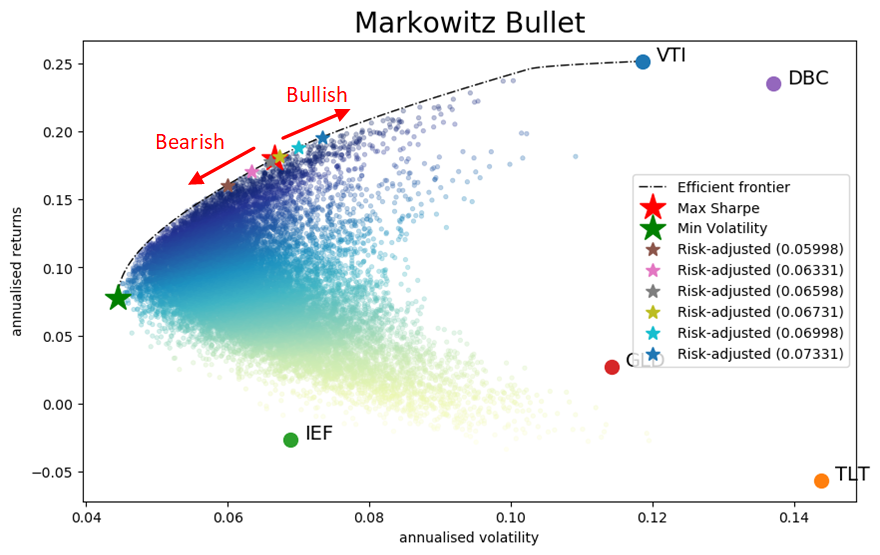
\includegraphics[width=8cm]{figure_smpt_markowitz.png}
    \caption{Illustration of sentiment-adjusted MPT on Markowitz Bullet \label{figure_smpt_markowitz}}
\end{figure}

Simulation is performed over the backtesting period and used to calculate a fitness score, F, which depends on our objective. We define three possible objectives - (i) maximise cumulative returns, (ii) maximise Sharpe Ratio, and (iii) minimise volatility, during the training period. These objectives correspond to different risk profiles for investors.

Optimisation via GA is performed based on the simplest evolutionary algorithm presented by Fogel et al. \cite{back2018evolutionary}, with crossover rate of 0.5 and mutation rate of 0.2. Multiple runs are performed for each combination of "Decision Points" in Fig \ref{figure_overall}, with varying population size, number of generations, and random seed.


\section{Experimental results}
\label{sec:experimental results}

We compare the various traditional portfolio optimisation techniques for our two different universes, and calculate cumulative returns, annual return, annual volatility, maximum drawdown, and Sharpe ratio. The Sharpe ratio of a portfolio is the ratio of mean risk-free excess return (over risk-free rate, $R_f$) to its standard deviation, $\sigma$, as given in Eqn \ref{eqn_sharpe}. The maximum dropdown expresses the largest drop between a peak and valley in percentage, for the backtesting period.

\begin{equation}
\text{Sharpe Ratio} = \frac{\bar{R_p}-R_f}{\sigma} \label{eqn_sharpe}
\end{equation}

Using the asset-class-based portfolio, it can be seen that the traditional approaches are able to reduce maximum draw-down and annual volatility, and improve cumulative returns, as compared to buy-and-hold of the index, SPY (Fig \ref{figure_bm_aw}, Table \ref{tab:aw}). In contrast, using a sector-based portfolio, all approaches moved similarly regardless of the optimisation technique (Fig \ref{figure_bm_sector}), which suggested that it will not benefit much from optimisation. Hence, we decide to focus our efforts on only the asset-based portfolio for the subsequent experiments.

\begin{figure}[tbh]
    \begin{subfigure}[t]{8cm}
        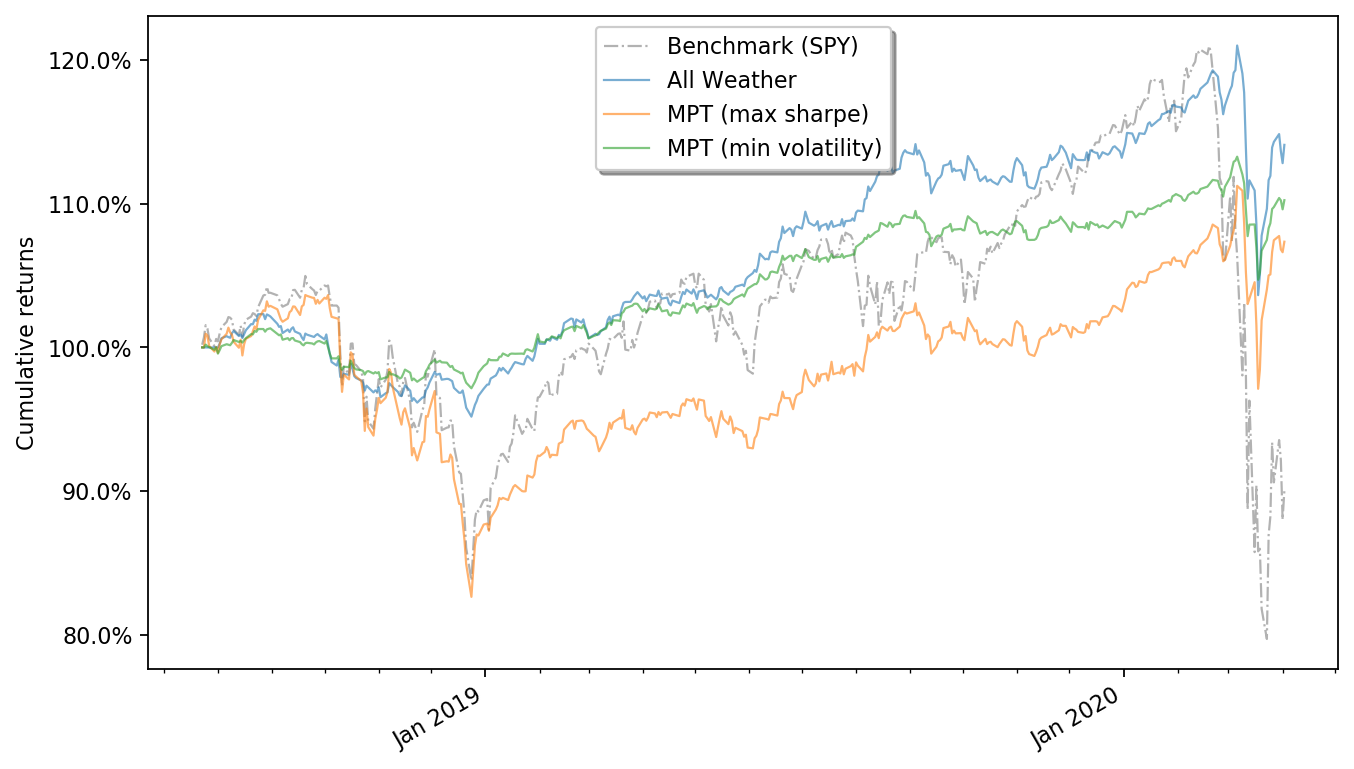
\includegraphics[width=8cm]{figure_benchmark_all_weather.png}
        \caption{Asset-class-based All-Weather portfolio \label{figure_bm_aw}}
    \end{subfigure}
    \begin{subfigure}[t]{8cm}
        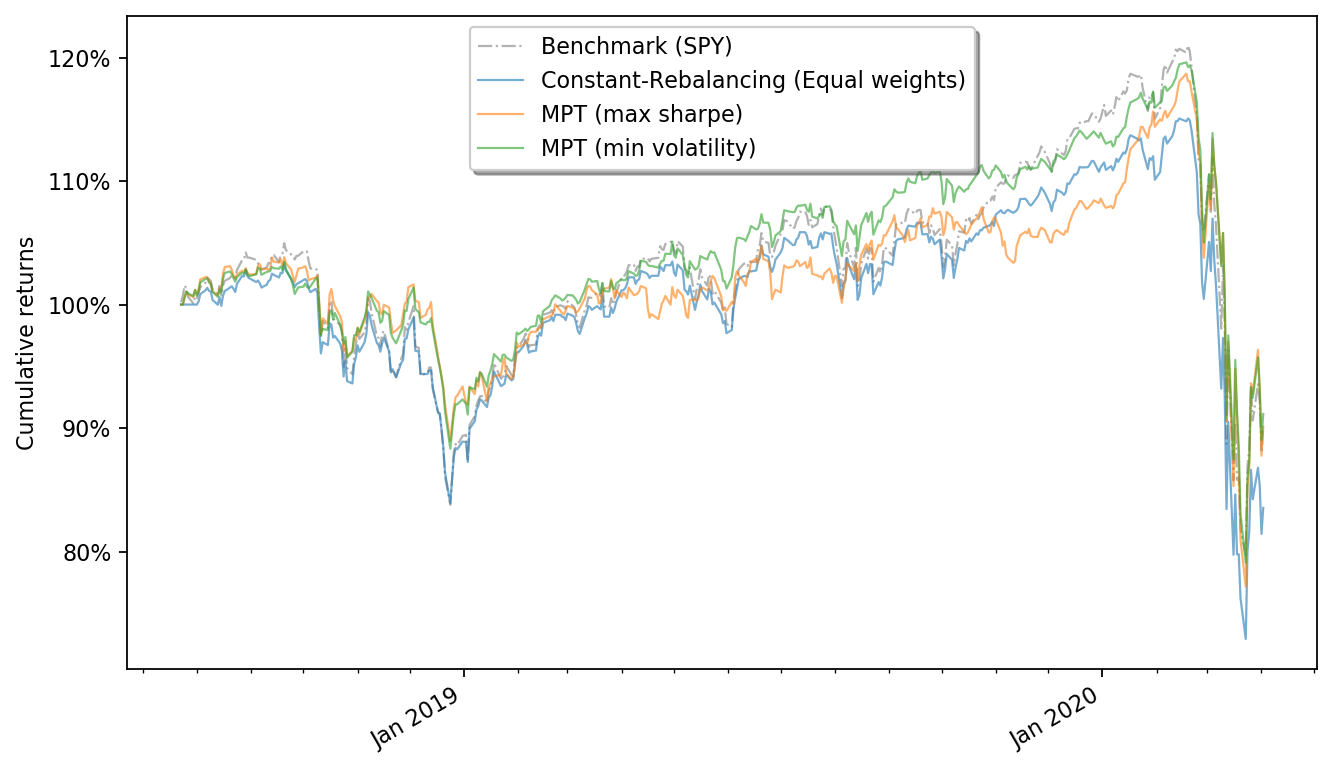
\includegraphics[width=8cm]{figure_benchmark_sectors.png}
        \caption{Sector-based SPDR sector ETFs portfolio\label{figure_bm_sector}}
    \end{subfigure}
\caption{Comparison of traditional approaches for the period of August 2018 to April 2020 \label{figure_bm}}
\end{figure}

\begin{table}[tbh]
  \centering
  \caption{Comparison of end performance for asset-class-based portfolio}
    \begin{tabular}{|p{4.4em}|r|r|r|r|}
    \toprule
    Metric & \multicolumn{1}{p{3em}|}{Baseline\newline{}(SPY)} & \multicolumn{1}{p{3em}|}{All-\newline{}Weather} & \multicolumn{1}{p{3em}|}{MPT\newline{} (max Sharpe)} & \multicolumn{1}{p{3em}|}{MPT \newline{}(min volatility)} \\
    \midrule
    Cumulative\newline{} returns & -11.26\% & \textbf{14.09\%} & 7.35\% & 10.24\% \\
    \midrule
    Annual\newline{}return & -6.78\% & \textbf{8.07\%} & 4.27\% & 5.91\% \\
    \midrule
    Annual\newline{}volatility & 25.21\% & 8.64\% & 12.49\% & \textbf{5.03\%} \\
    \midrule
    Max\newline{}drawdown & -34.11\% & -14.35\% & -20.26\% & \textbf{-7.56\%} \\
    \midrule
    Sharpe \newline{}ratio & -0.15 & 0.94  & 0.4   & \textbf{1.17} \\
    \bottomrule
    \end{tabular}%
  \label{tab:aw}%
\end{table}%

Tweets from various accounts are web scraped and converted to sentiments using VADER and FinBERT. In a random sampling of tweets, it is found that in most cases, FinBERT is able to score tweets more appropriately than VADER. Hence, while VADER is supposed to be suitable for social media, it is not good enough for finance related tweets. Some example tweets and sentiments are shown in Table \ref{tab:tweets_vader_finbert}.

We check for synchrony between daily stock data and the day-aggregated tweet sentiments during volatile periods, using Pearson correlation with time-shifting. In particular, it is found that tweet sentiments from CNBC (@cnbc) gave strong correlation with near-zero lag against SPY stock data. There is also some negative correlation between Donald Trump's (@realDonaldTrump) tweet sentiments and SPY (Fig \ref{figure_pearson}), which is similar to the findings by Brans and Scholtens \cite{DonaldTrumpTwitter}. Since @cnbc gives good correlation, the subsequent experiments are narrowed to using only their tweets.

\begin{table}[tbh]
  \centering
  \caption{Some example tweets sentiment-analysed with VADER and FinBERT}
    \begin{tabular}{|p{12em}|r|r|}
    \toprule
    Tweet & \multicolumn{1}{p{3em}|}{VADER} & \multicolumn{1}{p{3em}|}{FinBERT} \\
    \midrule
    JUST IN: U.S. weekly jobless claims surge to more than 6.6 million, vs. 3.1 million expected. & \textcolor[rgb]{ 1,  0,  0}{0} & -0.0689 \\
    \midrule
    The World Health Organization has declared the coronavirus outbreak a global pandemic & \textcolor[rgb]{ 1,  0,  0}{0} & -0.1286 \\
    \midrule
    Sometimes, the best thing to do is nothing. And according to Duke University behavioral economist @danariely, nothing is exactly what most investors should do during the coronavirus outbreak & \textcolor[rgb]{ 1,  0,  0}{0.6369} & -0.0115 \\
    \midrule
    The Chinese government has deliberately underreported the total number of coronavirus cases and deaths in the country, the U.S. intelligence community reportedly told the White House & \textcolor[rgb]{ 1,  0,  0}{0.5267} & -0.6744 \\
    \midrule
    European stocks just posted their worst quarter since 2002 & \textcolor[rgb]{ .129,  .129,  .129}{-0.6249} & \textcolor[rgb]{ .129,  .129,  .129}{-0.6510} \\
    \midrule
    Moody's cuts outlook on \$6.6 trillion US corporate debt pile to 'negative'  & \textcolor[rgb]{ .129,  .129,  .129}{-0.5719} & \textcolor[rgb]{ .129,  .129,  .129}{-0.9144} \\
    \bottomrule
    \end{tabular}%
    \
    Note: Red denotes sentiments that are deemed incorrect
  \label{tab:tweets_vader_finbert}%
\end{table}%

\begin{figure}[tbh]
    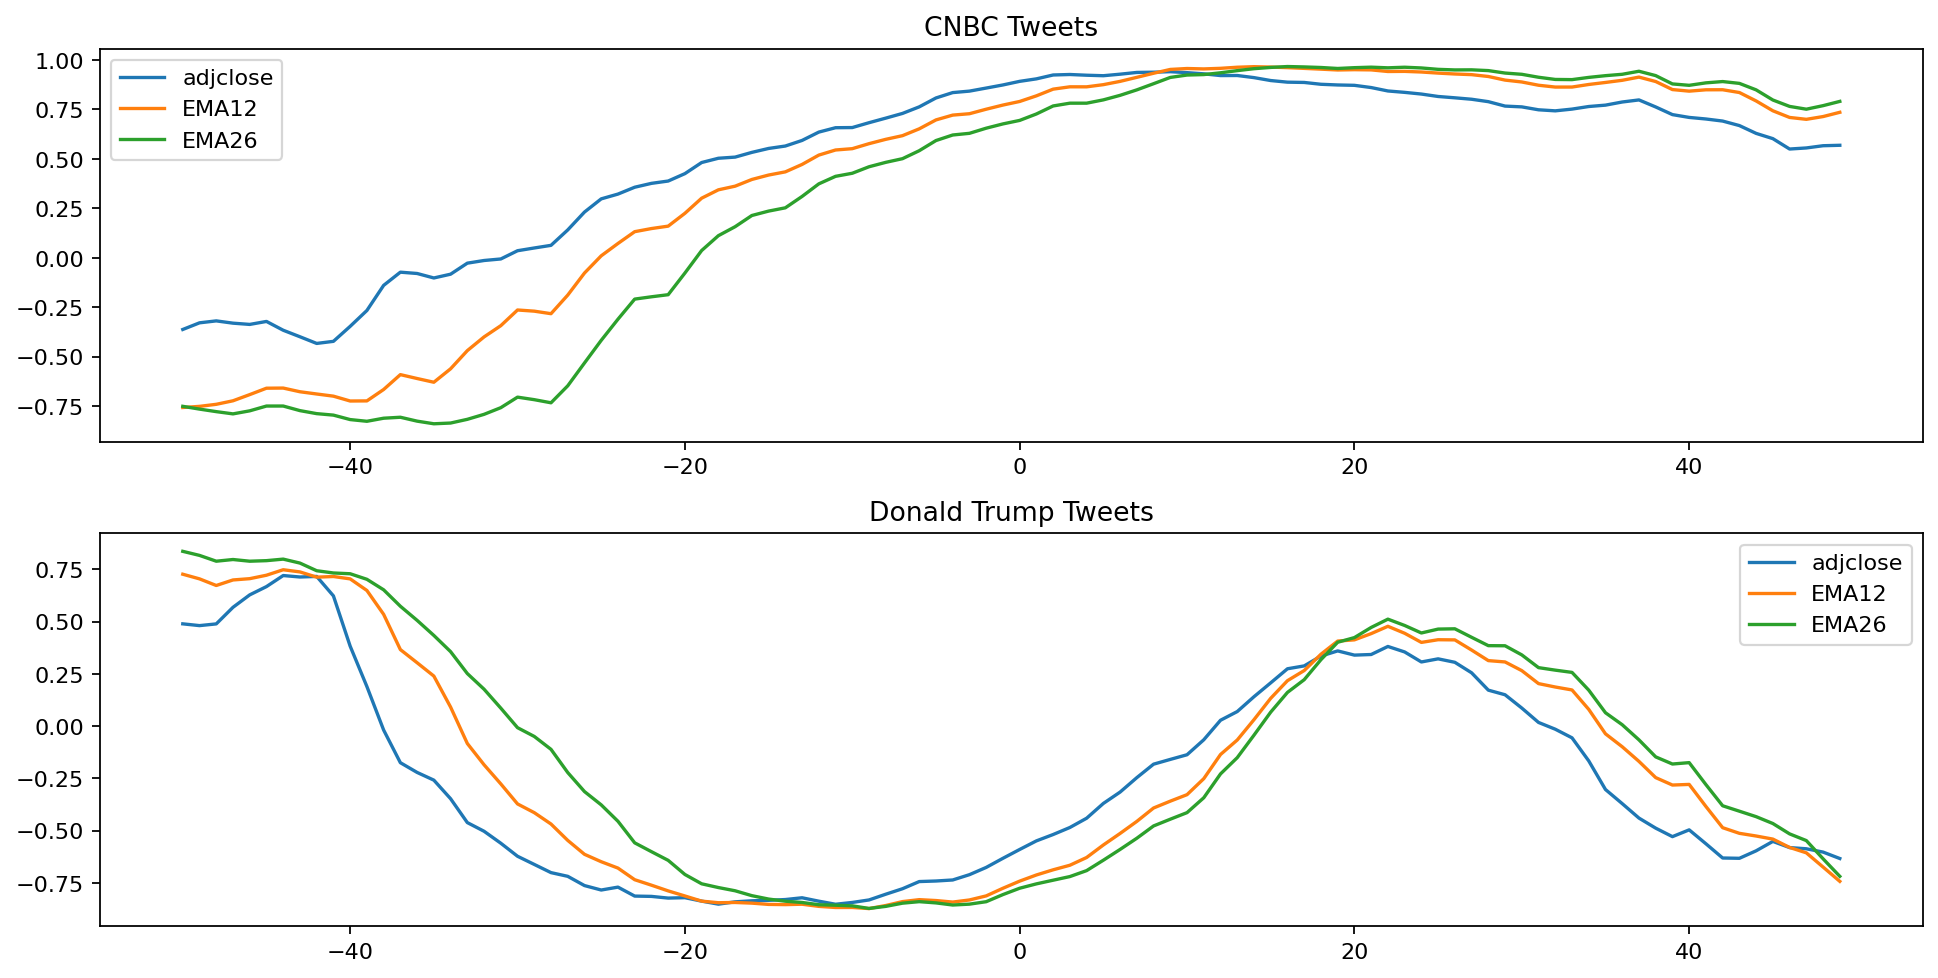
\includegraphics[width=8cm]{figure_pearson_coeff.png}
    \caption{Pearson coefficient against day-shifts for CNBC and Donald Trump's tweets \label{figure_pearson}}
\end{figure}


As a proof of concept, we initially try a single-asset portfolio of only SPY and add a simple modification function, M, that takes CNBC sentiments into account, similar to Table \ref{table_crb_mod}, which we term ``Sentimental SPY" portfolio. Even with a single asset, cumulative returns are improved compared to buy-and-hold SPY, as it is able to exit the market when sentiments are negative (Fig \ref{figure_sspy_vs_spy}). This means that the portfolio holds a lot of uninvested cash during volatile period, which to the average investor may be overly conservative (Fig \ref{figure_sspy_allocation}).


\begin{figure}[tbh]
\begin{subfigure}[t]{8cm}
    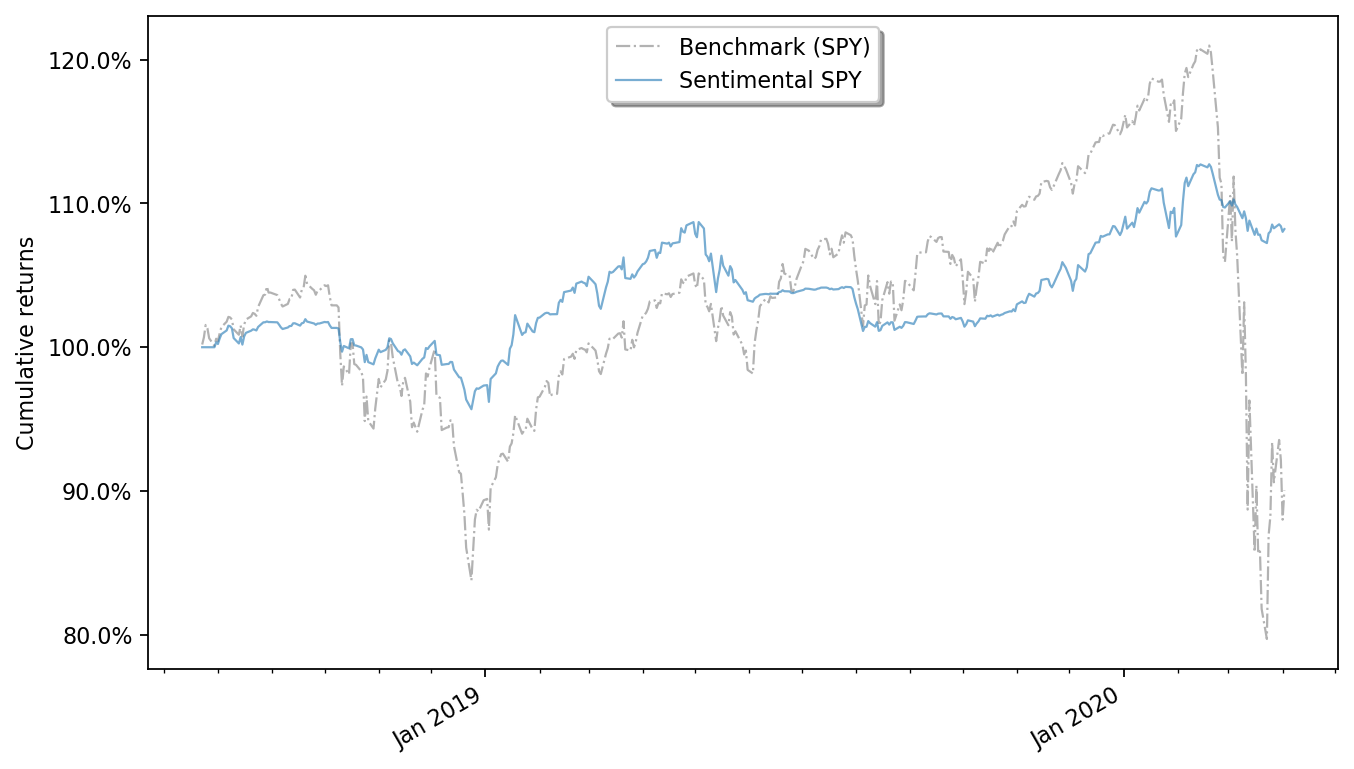
\includegraphics[width=8cm]{figure_benchmark_spy.png}
    \caption{Sentimental-SPY compared with SPY benchmark \label{figure_sspy_vs_spy}}
\end{subfigure}
\begin{subfigure}[t]{8cm}
    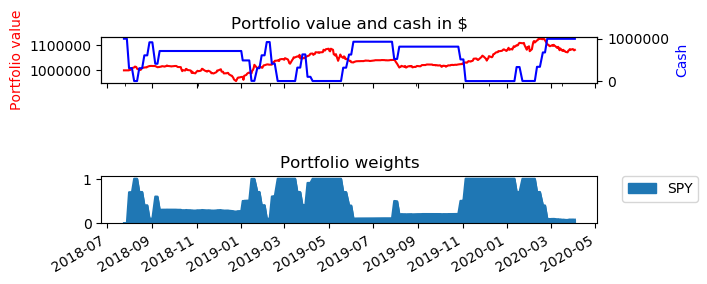
\includegraphics[width=8cm]{figure_analyse_sent_spy.png}
    \caption{Sentimental-SPY Portfolio allocation and value \label{figure_sspy_allocation}}
\end{subfigure}
\caption{Sentimental-SPY Portfolio \label{figure_sspy}}
\end{figure}

For a constant-rebalanced All-Weather portfolio, we use sentiments as trading signals to adjust allocation, which we term ``Sentimental All-weather" (SAW) portfolio. Initially, we attempted to use the raw sentiment score in the modification function (index 1 and 2 of Table \ref{table_crb_mod}); but portfolio rebalancing was highly unstable, hence a simple delta was used based on the MACD sentiment (index 3). We optimise parameters using GA over the training period of August 2018 to December 2019 for multiple runs, over three different objectives (maximum Sharpe, maximum cumulative returns, minimum volatility), rebalancing weekly. From Fig \ref{figure_saw}, we can see that in all runs, SAW performed better than buy-and-hold SPY, and frequently out-performed original All-Weather portfolio, which lends credence to its feasibility as an improved portfolio algorithm.

With the same All-Weather portfolio, we perform MPT optimisation and modify the volatility as given in Eqn \ref{eqn_smpt} to derive sentiment-adjusted weights, which we term ``Sentimental MPT" (SMPT) portfolio, and likewise optimised parameters using GA. SMPT models tend to converge to certain performance that fared worse for the out-of-sample period (as seen from Fig \ref{figure_smpt}), and only slightly better than MPT (Max Sharpe) for the entire period.

The performance metrics for out-of-sample data of (i) the best two SAW models for each objective, (ii) best SMPT model, and (iii) the baselines, are summarised in Table \ref{tab:saw_smpt}. We conclude that SAW optimised for minimum volatility (SAW-MV, model MV200-5-244) is able to achieve improved annual volatility, maximum drawdown and slightly higher cumulative returns, as compared to the original All-Weather portfolio. In addition, SAW optimised for maximum cumulative returns (SAW-MR, model MR100-10-0) is able to achieve significantly higher cumulative returns and Sharpe ratio, but had slightly higher volatility.


\begin{figure}
\begin{subfigure}[t]{8cm}
    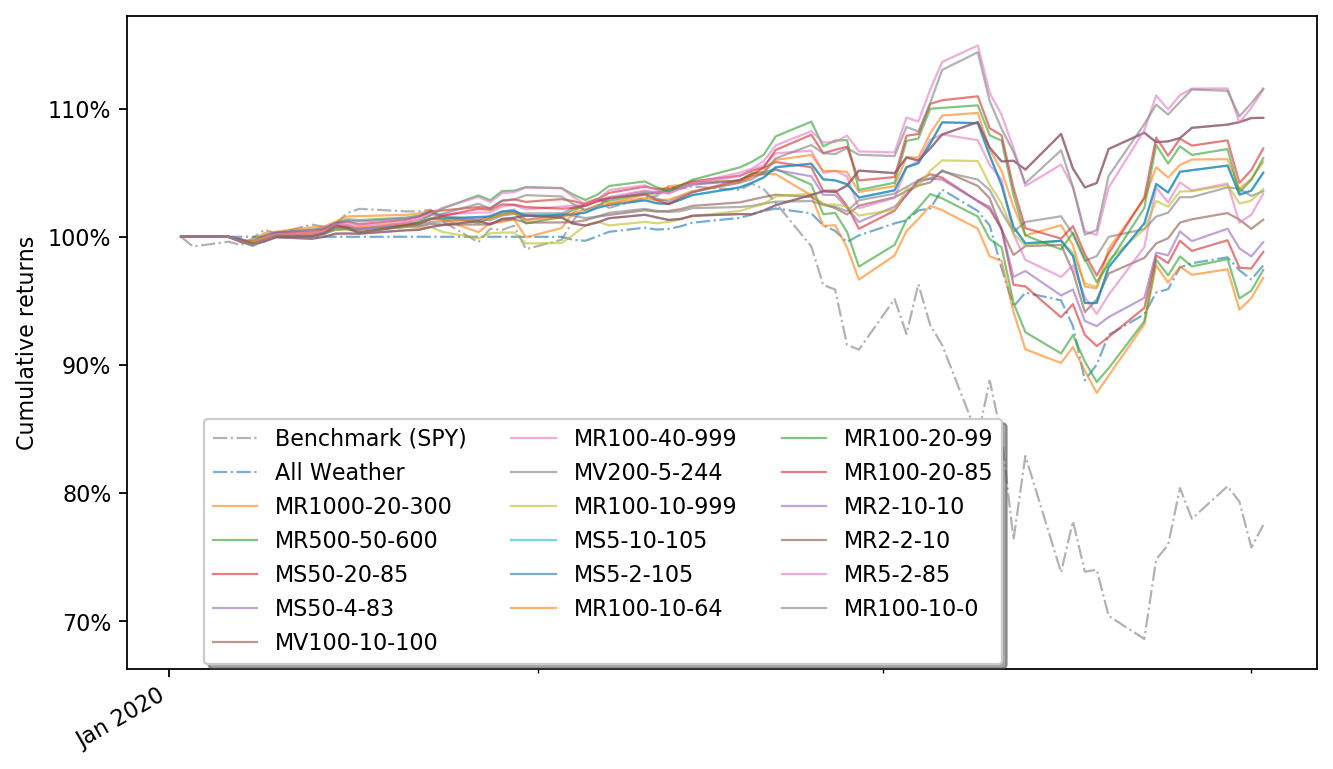
\includegraphics[width=8cm]{figure_saw.png}
    \caption{Sentimental All-Weather (SAW) portfolio \label{figure_saw}}
\end{subfigure}
\begin{subfigure}[t]{8cm}
    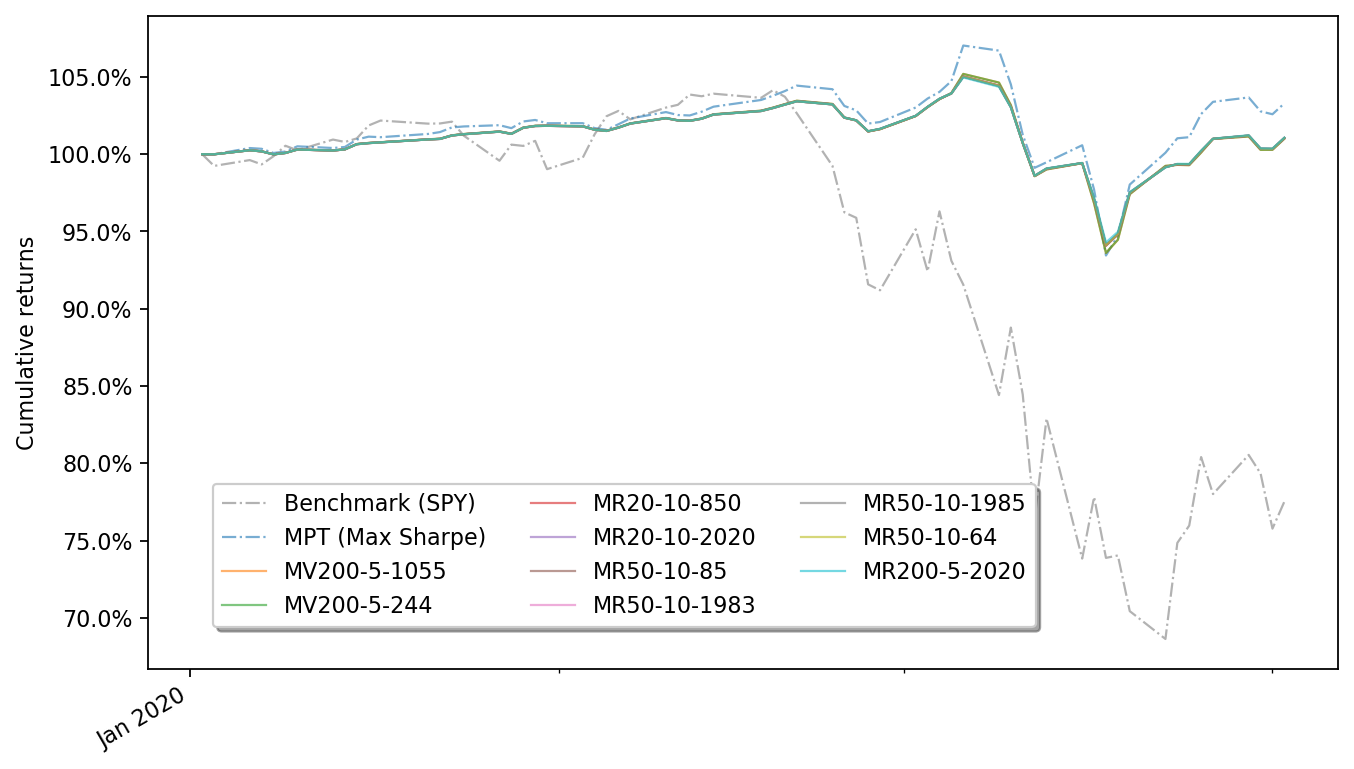
\includegraphics[width=8cm]{figure_smpt.png}
    \caption{Sentimental MPT (SMPT) portfolio \label{figure_smpt}}
\end{subfigure}
\caption{Comparison of Sentiment-adjusted portfolios on out-of-sample data \label{figure_saw_smpt}}

\end{figure}

\begin{table*}[htbp]
  \centering
  \caption{Comparison  of  performance for out-of-sample data for SAW and SMPT with baselines, on All-Weather portfolio}
    \begin{tabular}{|p{4em}|r|r|r|r|r|r|r|r|r|r|}
    \toprule
    \multicolumn{1}{|l|}{} & \multicolumn{1}{p{3.2em}|}{\cellcolor[rgb]{ .906,  .902,  .902}Baseline (SPY)} & \multicolumn{1}{p{3.2em}|}{\cellcolor[rgb]{ .906,  .902,  .902}CRB} & \multicolumn{1}{p{3.2em}|}{\cellcolor[rgb]{ .906,  .902,  .902}MPT (Max Sharpe)} & \multicolumn{1}{p{3.2em}|}{MPT MR200-5-2020} & \multicolumn{1}{p{3.2em}|}{MV100-10-100} & \multicolumn{1}{p{3.2em}|}{\textbf{MV200-5-244}} & \multicolumn{1}{p{3.2em}|}{MS5-10-105} & \multicolumn{1}{p{3.2em}|}{MS5-2-105} & \multicolumn{1}{p{3.2em}|}{MR100-20-99} & \multicolumn{1}{p{3.2em}|}{\textbf{MR100-10-0}} \\
    \midrule
    Cumulative returns & -23.60\% & -2.24\% & 3.29\% & 1.07\% & 1.34\% & 3.55\% & 5.00\% & 5.00\% & 6.14\% & \textbf{11.57\%} \\
    \midrule
    Annual return & -65.36\% & -8.53\% & 13.60\% & 4.29\% & 5.37\% & 14.73\% & 21.18\% & 21.18\% & 26.46\% & \textbf{53.87\%} \\
    \midrule
    Annual volatility & 55.05\% & 17.77\% & 18.01\% & 13.22\% & 13.09\% & \textbf{9.40\%} & 18.93\% & 18.93\% & 23.90\% & 21.22\% \\
    \midrule
    Max drawdown & -34.11\% & -14.35\% & -12.70\% & -10.17\% & -10.52\% & \textbf{-6.64\%} & -12.94\% & -12.94\% & -12.51\% & -12.45\% \\
    \midrule
    Daily value at risk & -7.30\% & -2.27\% & -2.21\% & -1.65\% & -1.63\% & \textbf{-1.13\%} & -2.30\% & -2.30\% & -2.91\% & -2.49\% \\
    \midrule
    Sharpe ratio & -1.65 & -0.41 & 0.8   & 0.38  & 0.46  & 1.51  & 1.11  & 1.11  & 1.1   & \textbf{2.14} \\
    \bottomrule
    \end{tabular}%

  \label{tab:saw_smpt}%
  \
  Note: Objective functions are MV, MS and MR where MV - Minimum Volatility, MS - Maximum Sharpe Ratio, MR - Maximum (Cumulative) Returns. Naming convention is [Objective][population size]-[number of generations]-[seed]
\end{table*}%

\section{Robo-advisor system}
\label{sec:robo}

Django is chosen as the web development framework to build our robo-advisor as it is one of the most popular open-source free web development tools, has a short learning curve, and is catered for rapid development \cite{vincent2020django}. In order to accelerate development even further, Django project skeleton provided by \href{https://django-edge.readthedocs.io/en/latest/}{Django Edge v2.2} is used. The prototype is deployed in Heroku.

We create a custom model class, Profile, to store and retrieve each investor's details, such as asset transfers, gross asset value, and available cash in account. For portfolio details, we choose to use a Pickle object as the structure of the portfolios is complex.

Our robo-advisor has the following core functionalities - (i) Basic user management - sign up and log in, (ii) Summary page showing current account balance, earnings, portfolio asset value, etc, (iii) Add and withdraw funds (virtual funds, no actual interface with real money), (iv) Portfolio management - compare, buy and sell portfolios. The list of portfolios is easily configurable from a spreadsheet, and includes SPDR sector ETFs, and All-Weather ETFs, SAW and SMPT portfolios. The overall user and system flows are shown in Fig \ref{figure_django}.

In order to categorise the portfolios based on risk, it is useful to use 99\%-Value-at-Risk (VaR) shown in Eqn \ref{eqn_var}. For example, a 99\%-VaR of -1.5\% will mean that there is a 99\% chance of not losing more than 1.5\% for the given time period. For simplicity, we classified risk into the following categories in Eqn \ref{eqn_risk}.

\begin{equation}
\text{99\%-VaR} = \bar{R_p} - 2.326\sigma  \label{eqn_var}
\end{equation}

\begin{equation} \label{eqn_risk}
\text{risk} = \begin{cases}
  \text{``low"}, &\text{VaR $>$ -10\%}  \\
  \text{``medium"}, &\text{VaR $>$ -20\%}  \\
  \text{``medium-high"}, &\text{VaR $>$ -30\%}  \\
  \text{``high"}, &\text{VaR $\leqslant$ -30\%} \\
\end{cases}
\end{equation}

\begin{figure}[htbp]
    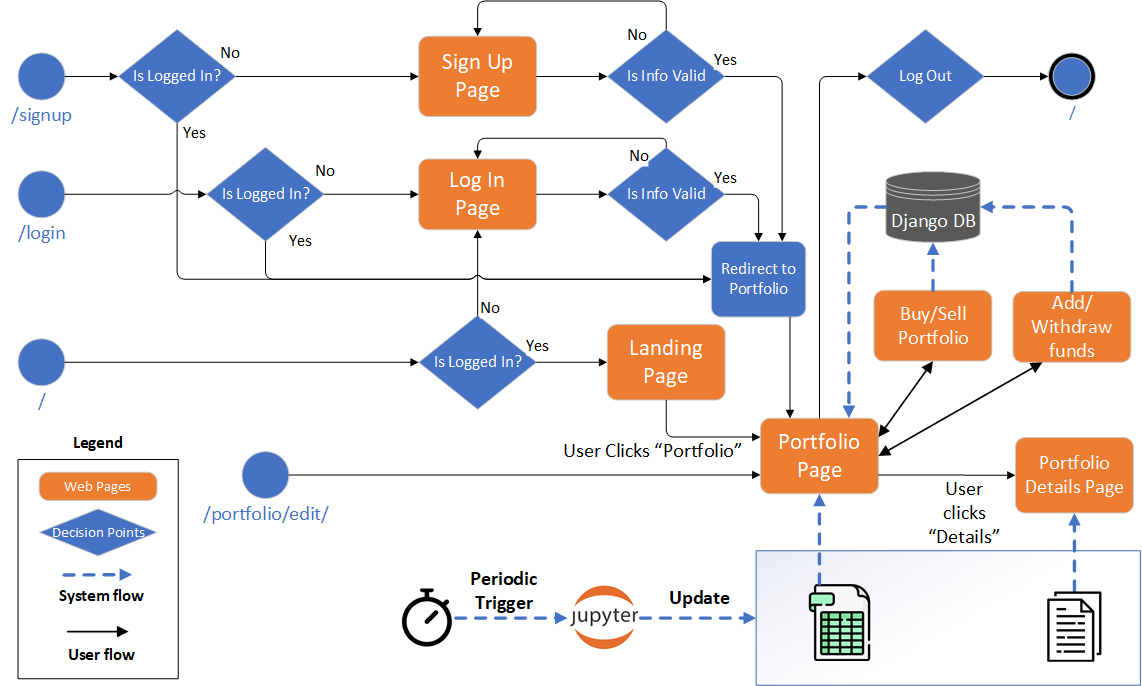
\includegraphics[width=8cm]{figure_django_architecture.png}
    \caption{User and system flow for Django robo-advisor app\label{figure_django}}
\end{figure}

\section{Conclusion}
\label{sec:conclusions}

Our proposed hybrid approach of using traditional portfolio techniques together with Twitter sentiments can improve portfolio performance, when optimised using GA for different objectives such as maximising cumulative returns or minimising volatility. The models proposed in this paper (SAW and SMPT) can be included as portfolios in a robo-advisor and easily deployed as an end-to-end system, using Fig \ref{figure_django}.

There are many simplification steps in this paper that may be expanded upon in future work. For example, in ETF selection, we can use more complicated algorithms to select the best performers for each asset class using rules or machine learning models. Sentiments can also be derived from a combination of different accounts, rather than just one, for more accurate daily sentiments. Our modification function can also be expanded upon to take in more inputs from other stocks or indices, such as the `fear' index (\^VIX), which has high readings when investors anticipate huge moves in the market. Other traditional algorithms such as HRP may also be added.

\bibliographystyle{IEEEbib}
\bibliography{references}

\end{document}
